\documentclass[a4paper,12pt]{article}

\providecommand{\No}{\textnumero}
%\setmarginsrb{3cm}{2cm}{1cm}{2cm}{0pt}{0mm}{0pt}{13mm}
\usepackage{indentfirst}
\sloppy
\setcounter{page}{0}
\clubpenalty = 10000
\widowpenalty = 10000

\usepackage[nottoc]{tocbibind} % Для того, чтобы список литературы отображался в оглавлении
\usepackage{verbatim} % Для вставок заранее подготовленного текста в режиме as-is

\usepackage[colorlinks,unicode]{hyperref}
\usepackage[affil-it]{authblk}
\usepackage[rgb]{xcolor}
\usepackage{float}
\usepackage{colortbl}
\hypersetup{				% Гиперссылки
    colorlinks=true,       	% false: ссылки в рамках
	urlcolor=blue           % на URL
}

%  Русский язык
\usepackage[T2A]{fontenc}			% кодировка
			% кодировка исходного текста
\usepackage[english,russian]{babel}	% локализация и переносы
\usepackage[utf8]{inputenc}

% Footnotes
\usepackage[bottom]{footmisc}

% Code
\usepackage{listings}
\usepackage{color}

\definecolor{dkgreen}{rgb}{0,0.6,0}
\definecolor{gray}{rgb}{0.5,0.5,0.5}
\definecolor{mauve}{rgb}{0.58,0,0.82}

\lstset{frame=tb,
  language=Python,
  aboveskip=3mm,
  belowskip=3mm,
  showstringspaces=false,
  columns=flexible,
  basicstyle={\small\ttfamily},
  numbers=none,
  numberstyle=\tiny\color{gray},
  keywordstyle=\color{blue},
  commentstyle=\color{dkgreen},
  stringstyle=\color{mauve},
  breaklines=true,
  breakatwhitespace=true,
  tabsize=3
}

% Subsubsections
\usepackage{titlesec}

\setcounter{secnumdepth}{4}

\titleformat{\paragraph}
{\normalfont\normalsize\bfseries}{\theparagraph}{1em}{}
\titlespacing*{\paragraph}
{0pt}{3.25ex plus 1ex minus .2ex}{1.5ex plus .2ex}

% Математика
\usepackage{amsmath,amsfonts,amssymb,amsthm,mathtools}
\usepackage{thmtools}
\usepackage{cases}

\usepackage{physics}
\usepackage{cleveref}

% Mathematical formating
\newtheorem{theorem}{Теорема}
\theoremstyle{definition}
\newtheorem{definition}{Определение}[section]
\renewcommand{\theoremautorefname}{теоремы}

% Add lemma support
\newtheorem{lemma}{Лемма}
\newtheorem{sublemma}{Лемма}[lemma]

\usepackage{wasysym}

\makeatletter
% Roman numbers support
\newcommand*{\rom}[1]{\expandafter\@slowromancap\romannumeral #1@}

% Derivative at point support
\newcommand{\at}[2][]{#1|_{#2}}

% Expectation support
\newcommand{\expect}{\operatorname{E}\expectarg}
\DeclarePairedDelimiterX{\expectarg}[1]{[}{]}{%
  \ifnum\currentgrouptype=16 \else\begingroup\fi
  \activatebar#1
  \ifnum\currentgrouptype=16 \else\endgroup\fi
}

\newcommand{\innermid}{\nonscript\;\delimsize\vert\nonscript\;}
\newcommand{\activatebar}{%
  \begingroup\lccode`\~=`\|
  \lowercase{\endgroup\let~}\innermid 
  \mathcode`|=\string"8000
}

\renewcommand\qedsymbol{$\blacksquare$}

\makeatother

\begin{document}

% НАЧАЛО ТИТУЛЬНОГО ЛИСТА
\begin{center}
\ \vspace{-2cm}

%
\includegraphics[width=0.5\textwidth]{msu.eps}\\

\includegraphics[width=0.5\textwidth]{img/msu.jpg}\\
{\scshape Московский государственный университет \\ имени М.В. Ломоносова}\\
Факультет вычислительной математики и кибернетики\\
Кафедра исследования операций

\vspace{4cm}

\textbf{{\Large Мирзоев Сергей Евгеньевич}}

\vspace{1cm}

{\Huge\bfseries
Оценка бессрочных опционов для случайных процессов со скачками\\}
\end{center}

\vspace{1cm}
\begin{center}
{\normalsize Выпускная квалификационная работа}
\end{center}

\vspace{2cm}

\vfill

\begin{flushright}
\normalsize
\textbf{Научный руководитель:}\\
доцент, к.ф.-м.н\\
Г.А. Белянкин\\
\textbf{Со-руководитель:}\\
доцент, к.ф.-м.н\\
В.В. Морозов
\end{flushright}

\vfill

\begin{center}
Москва, 2021
\end{center}

\enlargethispage{4\baselineskip}
\thispagestyle{empty} % выключаем отображение номера для этой страницы
\newpage

\thispagestyle{empty}

\newpage
\tableofcontents

\newpage

%%%%%%%%%%%%%%%%%%%%%%%%%%%%%%%%%%%%
%%%%%%%%%%%%% Введение %%%%%%%%%%%%%
%%%%%%%%%%%%%%%%%%%%%%%%%%%%%%%%%%%%
\section{Введение}

Разработка современных моделей ценообразования опционов началась с публикации Фишера Блэка и Майрона Шоулза в 1973 году \cite{bib:Black_Scholes}. Их работа навсегда изменила взгляд как практиков, так и теоретиков ценообразования производных ценных бумаг. Данная модель использовалась впоследствии многими авторами для оценки оптимального порога для бесконечного колл-опциона в модели Блэка - Шоулза \cite{bib:Perpetual_Mart1, bib:Perpetual_Mart2}. Впоследствии, как в прошлом веке \cite{bib:Musiela1997}, так и в наше время \cite{bib:BSModification} ряд авторов часто обращались к оригинальной статье и сумели развить модель Блэка-Шоулза, внеся в нее существенные дополнения, и в настоящее время можно говорить о существовании нескольких подходов к ценообразованию опционов.

Известно, что реальные финансовые данные имеют большую волатильность в течение определенного периода, а в другое время они имеют меньшую волатильность на рынке. Существуют модели, которые проводятся для воспроизведения эффекта кластеризации волатильности, такие как стохастическая волатильность и модели GARCH \cite{bib:GARCH}.  В данной работе более подробно рассмотренны аффинные модели стохастической волатильности и аффинной скачкообразной диффузии, которые представляют собой комбинацию моделей стохастической волатильности и скачкообразной диффузии.

Серьёзный вклад в создание моделей для оценки опционов и прочих дериватовов внесли Гербер и Шиу, наиболее заметными работами которых являются оценка опционов с помощью преобразования Эшера, где было показано, что преобразование Эшера также является эффективным методом оценки производных ценных бумаг, если логарифмы цен примитивных ценных бумаг подчиняются определенным стохастическим процессам со стационарными и независимыми приращениями \cite{bib:GerberShiu_Esscher}; а также статьи, где рассматривались актуарные подходы к оценке опционов \cite{bib:GerberShiu_Actuarial_1, bib:GerberShiu_Actuarial_2, bib:GerberShiu_Actuarial_3}. 

Вдохновением текущей работе же послужила более современная статья Гербера и Шиу \cite{bib:GerberShiu}, где была сделана оценка бесконечного опциона \textit{пут}, использующая модель процесса со скачками. В данной статье аналогичный результат будет получен для \textit{колл-опциона}. Как и в указанной статье, в данной работе рассматриваются две модели, в которых логарифм цены актива представляет собой смещённый сложный пуассоновский процесс\textsuperscript{\ref{sec:compound_poisson}}. Явные результаты получены для цен и оптимальных стратегий исполнения определенных бессрочных американских опционов на актив, в частности для бессрочного колл-опциона. В первой модели, в которой скачки цены актива направлены вверх, результаты получаются с использованием процесса - мартингала и условия гладкого сшивания. Во второй модели, в которой скачки идут вниз, показывается, что значение стратегии, соответствующее постоянной границе исполнения опциона удовлетворяет определенному уравнению обновления. Будет получена оптимальная стратегию исполнения, удовлетворяющая условию непрерывного сшивания. Кроме того, одна и та же модель может быть использована для определения цены на определенные параметры отмены. Наконец, было показано, как классическая модель геометрического броуновского движения может быть использована в качестве предела, а также, как она может быть встроена в обе модели.

%%%%%%%%%%%%%%%%%%%%%%%%%%%%%%%%%%%%
%%%%%%%% Постановка задачи %%%%%%%%%
%%%%%%%%%%%%%%%%%%%%%%%%%%%%%%%%%%%%

\section{Постановка задачи}

Пусть $S(t)$ - цена актива, например, акции, в момент времени $t \ge 0$. Мы предполагаем, что рынок риск-нейтрален\footnote{Нейтральность к риску — свойство предпочтений инвестора, отражающее его безразличие при выборе между средним ожидаемым выигрышем в некоторую лотерею и гарантированным выигрышем такой же величины. Если ситуация неопределенности обеспечивает такой же средний в смысле вероятностей ожидаемый выигрыш, что и некоторая гарантированная сумма, то инвестору все равно, что выбрать. Если ожидаемый выигрыш оказывается больше, то инвестор предпочтет ситуацию неопределенности, несмотря на риск проиграть при некотором исходе.}, следовательно, стоимость ценной бумаги - это математическое ожидание дисконтированных будущих платежей. В предположении, что по активу не выплачивается никаких дивидендов и что безрисковая мгновенная процентная ставка $r$ является положительной константой, случайный процесс $\{e^{-rt} S(t)\}$, представляющий собой дисконтированную цену актива  является мартингалом.

\subsection{Модель Блэка-Шоулза}

Напомним, что в модели Блэка-Шоулза стоимость акции представляется в виде:

\begin{equation}\label{eq:black_sholes_equation}
    S(t) = S(0) e^{\tilde{\alpha} t + \sigma Z(t)} = e^{ln S(0) + \tilde{\alpha} t + \sigma Z(t)}
\end{equation}

где $\tilde{\alpha} = \alpha - \frac{\sigma^2}{2}$, а $Z (t)$ - винеровский процесс. В рассматриваемыми нами моделями, будет рассмотрена стоимость акций для процесса со скачками.

Простота модели Блэка-Шоулза была достигнута путем принятия следующих допущений, что цена актива следует геометрическому броуновскому движению $\frac{dS(t)}{S(t)} = \mu dt + \sigma dW(t)$, где $W$ - броуновское движение, $\mu$ - среднее значение, также известное как дрейф, $\sigma$ представляет собой волатильность относительного изменения цены акций, а $S(t)$ - текущую цену акций. Также предполагается, что волатильность $\sigma$ изменения цены акций и безрисковая процентная ставка r являются постоянными.

\subsection{Модель со скачками цены}

Пусть $U(t) = \ln{S(t)}, t \ge 0$. Мы предполагаем, что $\{U(t), t \ge 0\}$ - процесс с независимыми и стационарными приращениями, с начальным значением $U(0) = \ln{S(0)} = \ln{s} = u$. Классическая модель цены акции является частным случаем, в котором $\{U(t)\}$ представляет собой винеровский процесс со сдвигом $\mu = r - \frac{\sigma ^ {2}}{2}$ и бесконечно малой дисперсией $\sigma ^ {2}$. 

В данной работе будут рассмотрены две модели:

\textbf{Модель \rom{1}:}\footnote{Заметим, что модель \rom{1} напоминает модель, которая используется для процесса избытка в классической теории риска.}
\begin{equation}\label{eq:model1_definition}
    U(t) = u + ct - Z(t)
\end{equation}

\textbf{Модель \rom{2}}: 
\begin{equation}\label{eq:model2_definition}
    U(t) = u - ct + Z(t)
\end{equation}

В обоих случаях $c > 0$ и является постоянной величиной, а $\{Z(t)\}$ представляет собой сложный пуассоновский процесс, определяемый параметром $\lambda > 0$ и распределением величин скачка. Заметим также, что скачки положительны.

\label{sec:positivityOfJumsAssumption} Для упрощения обозначений предположим, что распределения величин скачка
непрерывны с плотностью вероятности $p(x), x \ge 0$. 

\subsection{Некоторые факты из теории вероятностей}

Для удобства дальнейшего изложения приведём несколько определений, опираясь в частности на метидические пособия Ширяева \cite{bib:Shiryaev,bib:Shiryaev_Bulynski}.

\subsubsection{Фильтрация}

\begin{definition}[Сигма-алгебра]
    \label{def:sigma_algebra}
    Семейство $\Xi$ подмножеств множества $X$ называется $\sigma$-алгеброй, если оно удовлетворяет следующим свойствам:
    
    \begin{itemize}
        \item $\Xi$ содержит множество $X$ и пустое множество $\varnothing$.
        \item Если $E \in \Xi$, то и его дополнение $X \backslash E \in \Xi$
        \item Объединение или пересечение счётного подсемейства из $\Xi$ принадлежит $\Xi$
    \end{itemize}

\end{definition}

\begin{definition}[Фильтрация]
    \label{def:filtration}
    Фильтрация в теории случайных процессов — неубывающее семейство $\sigma$-алгебр\textsuperscript{\ref{def:sigma_algebra}}.
    
    Пусть дано вероятностное пространство $(\Omega,{\mathcal {F}},\mathbb {P})$ и подмножество числовой прямой $T\subset \mathbb {R}$. Семейство $\sigma$-алгебр $\{\mathcal {F}_{t}\}_{t\in T}$ такое, что:

    \begin{equation*}
        {\mathcal  {F}}_{s}\subset {\mathcal  {F}}_{t}\subset {\mathcal  {F}},\quad \forall s\leq t,\;s,t\in T,
    \end{equation*}
    
    называется фильтрацией вероятностного пространства $(\Omega,{\mathcal {F}},\mathbb {P})$.

\end{definition}

\begin{definition}[Естественная фильтрация]
    \label{def:natural_filtration}
    Пусть дан случайный процесс $\{X_{t}\}_{t\in T}$, определённый на некотором вероятностном пространстве. Определим:

    \begin{equation*}
        {\mathcal  {F}}_{t}^{X}=\sigma \{X_{s}\mid s\leq t,\;s\in T\},\quad t\in T.
    \end{equation*}
    
    Тогда семейство $\left\{{\mathcal  {F}}_{t}^{X}\right\}_{{t\in T}}$ является фильтрацией и называется естественной фильтрацией случайного процесса $\{X_{t}\}$.

\end{definition}

\begin{definition}[Мартингал]
    \label{def:martingale}
    Мартингал — такой случайный процесс, что наилучшим (в смысле математического ожидания) предсказанием поведения процесса в будущем является его настоящее состояние.
    
    Для мартингалов с непрерывным временем математическая формулировка следующая:
    
    Пусть есть вероятностное пространство $(\Omega ,{\mathcal {F}},\mathbb {P} )$ с заданной на нём фильтрацией $\{{\mathcal {F}}_{t}\}_{t\in T}$, где $T\subset \mathbb {R}$. Тогда случайный процесс $\{X_{t}\}_{t\in T}$ называется мартингалом относительно $\{{\mathcal {F}}_{t}\}$, если:
    
    \begin{itemize}
        \item $X_{t}$ измерима относительно ${\mathcal {F}}_{t}$ для любого $t\in T$.
        \item ${\mathsf {E}}|X_{t}|<\infty ,\quad t\in T$.
        \item ${\mathsf {E}}[X_{t}\mid {\mathcal {F}}_{s}]=X_{s}$ почти наверное, $\quad \forall s,t\in T,\;s\leq t.$
    \end{itemize}

    Если в качестве $\{{\mathcal {F}}_{t}\}$ взята естественная фильтрация ${\mathcal {F}}_{t}=\sigma \{X_{s}\mid s\leq t\}$, то $\{X_{t}\}$ называют просто мартингалом.
    
    Для пояснения определения на понятном примере, рассмотрим игру, при которой подбрасывается монета, и при выпадении «орла» игрок выигрывает 1 руб., а при выпадении «решки» проигрывает 1 руб. Тогда если монета уравновешена, то состояние игрока как функция количества игр является мартингалом.
    
    Винеровский процесс (это математическая модель броуновского движения) является мартингалом.

\end{definition}

Далее мы всюду будем рассматривать именно мартингалы с естественной фильтрацией 

\subsubsection{Сложный пуассоновский процесс}\label{sec:compound_poisson}

Перед тем, как далее исследовать предложенные модели, стоит уточнить, что такое сложный пуассоновский процесс, а также получить важные результаты, связанные с ним.

\begin{definition}[Сложный пуассоновский процесс]
    \label{def:compound_poisson}
    Процесс $\{X_t, t \ge 0\}$ называется \textbf{сложным процессом Пуассона}, если мы можем записать его как:
    
    \begin{equation}
        X_t = \sum_{i=1}^{N_t} Y_i,
    \end{equation}
    
    где $\{N_t, t \ge 0\}$ - процесс Пуассона, а $\{Y_n\}_{n \ge 1}$ - семейство случайных независимых v. с тем же распределением, которые также независимы от $\{N_t, t \ge 0\}$.
\end{definition}

\begin{definition}\label{def:moment_generating_function}
Через \textbf{производящую функцию моментов} случайной величины $X$ будем обозначать:
    \begin{equation*}
        M_X(\alpha) = \expect{e^{\alpha X}}
    \end{equation*}
\end{definition}

\begin{lemma}\label{thm:thm2_moment_generating_function}
Производящая функция сложного Пуассоновского процесса $\{X(t)\}$ равна:

\begin{equation}\label{eq:moment_generating_for_poisson}
     M_{X(t)}(\alpha) = e^{\lambda t \left(M_{Y_1}(\alpha) - 1\right)}
\end{equation}

\end{lemma}

\begin{proof}

Распишем производящую функцию моментов для обобщенного Пуассоновского процесса:

\begin{equation*}
     M_{X_t}(\alpha) = \expect[\big]{e^{\alpha X_t}} = \expect[\big]{e^{\alpha \sum_{i=1}^{N_t} Y_i}}
\end{equation*}

Также заметим, что распределение $N_t$ нам известно:

\begin{equation}\label{eq:thm2_moment_generating_function_eq1}
     \expect[\big]{e^{\alpha \sum_{i=1}^{N_t} Y_i}} = \sum_{m=0}^{\infty} \expect[\big]{e^{\alpha \sum_{i=1}^{m} Y_i}} P(N_t = m) = \sum_{m=0}^{\infty} \expect[\big]{e^{\left(\alpha \sum_{i=1}^{m} Y_i\right)}} \frac{(\lambda t)^{m} e^{-\lambda t}}{m!}
\end{equation}

Так как случайные величины $Y_i$ независимы и одинаково распределены, верно:

\begin{equation}\label{eq:thm2_moment_generating_function_eq2}
     \expect[\big]{e^{\alpha \sum_{i=1}^{m} Y_i}} = \expect[\big]{\prod_{i=1}^{m} e^{\alpha Y_i}} = \prod_{i=1}^{m}  \expect[\big]{e^{\alpha Y_i}} = \prod_{i=1}^{m}  \expect[\big]{e^{\alpha Y_1}} = \left( \expect[\big]{e^{\alpha Y_1}} \right)^{m}
\end{equation}

Далее необходимое получается при подстановке \eqref{eq:thm2_moment_generating_function_eq1} и \eqref{eq:thm2_moment_generating_function_eq2} в цепочку уравнений:

\begin{equation*}
\begin{split}
    \sum_{m=0}^{\infty} \expect{e^{\left(\alpha \sum_{i=1}^{m} Y_i\right)}} \frac{(\lambda t)^{m} e^{-\lambda t}}{m!} &= \sum_{m=0}^{\infty} \left(\expect{e^{\alpha Y_1}}\right)^{m} \frac{(\lambda t)^{m} e^{-\lambda t}}{m!} =\\
    = \sum_{m=0}^{\infty} (M_{Y_1} (\alpha))^{m} \frac{(\lambda t)^{m} e^{-\lambda t}}{m!} &= \sum_{m=0}^{\infty} \frac{(M_{Y_1} (\alpha) \lambda t)^{m}}{m!} e^{-\lambda t} =\\
    = e^{\left(M_{Y_1} (\alpha) \lambda t\right)} e^{-\lambda t} &= e^{\lambda t \left(M_{Y_1}(\alpha) - 1\right)}
\end{split}
\end{equation*}

\end{proof}

\subsubsection{Свойство отсутствия памяти}

\begin{definition}\label{def:memoryless_distr}
    В ТВиМС \textit{отсутствие памяти} является свойством определенных вероятностных распределений. Обычно это относится к случаям, когда распределение «время ожидания» до определенного события не зависит от того, сколько времени уже прошло (если время ожидания автобуса распределено экспоненциально, то нет разницы: ждёте ли вы уже 10 минут или только пришли – вероятность, что автобус придёт через 5 минут остаётся той же).

    Точное определение: случайная величина Х называется величиной без памяти, если любых $s,t \ge 0$ выполняется:
    
    \begin{equation}\label{eq:memoryless_d_prob}
        P(X > s + t\textup{ | }X > s)  = P(X > t)
    \end{equation}
    
\end{definition}

Примером распределения не имеющего памяти является экспоненциальное распределение с параметром $\lambda$: 
    
\begin{equation}\label{def:exponential_distribution}
    f_X (t) = \lambda e^{-\lambda t}, \textbf{\ при\ } t \ge 0
\end{equation}

\begin{theorem}
Если $X$ экспоненциально распределённая случайная величина с параметром $\lambda > 0$, то $X$ является случайной величиной без памяти.
\end{theorem}

\begin{proof}
Для начала применим формулу условной вероятности:

\begin{equation*}
    P (X > x + a\textup{ | }X > a) = \frac{P (\{X > x + a\}\And\{X > a\})}{P(X > a)}
\end{equation*}

Учитывая, что $\{X > a\} \in \{X > x + a\}$ для $x \ge 0$:

\begin{equation*}
    \frac{P (\{X > x + a\}\And\{X > a\})}{P(X > a)} = \frac{P(X > x + a)}{P(X > a)}
\end{equation*}

Выражая вероятность через функцию распределения:

\begin{equation*}
    \frac{P(X > x + a)}{P(X > a)} = \frac{1 - F_X(x + a)}{1 - F_X(a)}
\end{equation*}

Подставим формулу для функции распределения \eqref{def:exponential_distribution}:

\begin{equation*}
    \frac{1 - F_X(x + a)}{1 - F_X(a)} = \frac{e^{-\lambda (x + a)}}{e^{-\lambda a}} = e^{-\lambda x} = P(X > x)
\end{equation*}

Итак, для экспоненциального распределения:

\begin{equation*}
    P (X > x + a\textup{ | }X > a) = P(X > x)
\end{equation*}

\end{proof}

\subsubsection{Теорема о преобразовании свободного выбора}

Пусть $\xi (t)$ - случайный процесс, являющийся мартингалом, т.е.:

\begin{equation*}
    \expect{\xi (t)|\xi(0)} = \xi(0)
\end{equation*}

Если правило предъявления опциона $T_L$ ограничено, т.е. $T_L \le T$ при некотором $T$, то $\expect{\xi (t)|\xi(0)} = \xi(0)$.

В нашем случае $\tau$ может принимать значение $\infty$. Он называется марковским моментом.

Если $\mathbb{P} (\tau < \infty) = 1$, то марковский момент называется моментом остановки. Если $\tau = \infty$, то $\xi (\infty) = 0$. 

Докажем теорему преобразования свободного выбора для марковских моментов.

\begin{theorem}\label{thm:OptSamplTheorem}
Для любого марковского момента $\xi$ выполнено неравенство $\expect{\xi (\tau) | \xi (0)} \le \xi(0)$. 
\end{theorem}

\begin{proof}

Рассмотрим случайные величины:

\begin{equation*}
    \eta = 1_{\{ \tau < \infty \}} \xi (\tau)
\end{equation*}
\begin{equation*}
    \eta_n = 1_{\{ \tau < n \}} \xi (\tau), \textup{\ при\ } n \in \mathbb{N}
\end{equation*}

Заметим, что:

\begin{equation*}
    \{\tau < n\} \in \{\tau < n + 1\}
\end{equation*}

А значит $1_{\{ \tau < n \}} \le 1_{\{ \tau < n + 1 \}}$ (с равенством при $\xi (\tau) = 0$). Как следствие, $\eta_n \le \eta_{n + 1}$ при всех $n \in \mathbb{N}$.

Также отметим очевидный факт $\lim_{n \to \infty} \eta_n = \eta$, иначе говоря, $\eta_n$ монотонно сходится к $\eta$.

Имеем $\expect {\eta (\tau)} = \expect {1_{\{ \tau < \infty \}} \xi (\tau)} + \expect {1_{\{ \tau = \infty \}} \xi (\infty)} = \expect {\eta}$, поскольку $\xi (\infty) = 0$.

Положим $\tau \wedge n = min (\tau, n)$.

\begin{equation*}
    \expect {\eta_n} = \expect {1_{\{ \tau < n \}} \xi (\tau)} \le \expect {1_{\{ \tau < n \}} \xi (\tau)} + \expect {1_{\{ \tau \ge n \}} \xi (n)} = \expect {\xi (\tau \wedge n)} = \xi (0)
\end{equation*}

Последний результат вытекает из теоремы о преобразовании свободного выбора (Подробнее: \ref{thm:OptSamplTheorem}). 

Итак, $\expect {\eta_n} \le \xi (0)$, при $\forall n \in \mathbb{N}$.

Переходя в этом неравенстве к пределу при $n \to \infty$, получим $\expect {\eta} = \expect {\xi (\tau)} \le \xi (0)$

\end{proof}

\subsection{Некоторые факты из экономической теории}

Также для лучшего понимания экономического смысла рассматриваемых моделей разберём следующие экономические факты.

\begin{definition}[Шорт, короткая позиция]
    \label{def:short_position}
    \textbf{Продажа без покрытия или торговля в шорт} --- продажа ценных бумаг, товаров или валюты, которыми торговец на момент продажи не владеет. Такая операция возможна, если условия контракта предусматривают его исполнение (поставку) через некоторое время или при маржинальной торговле, когда разрешено продавать взятый у брокера в кредит товар с предполагаемой последующей покупкой аналогичного товара и возврата кредита в натуральном (товарном) виде. Торговец надеется, что цена упадёт и он сможет дешевле выкупить ранее проданный товар. Этот механизм обеспечивает возможность получать прибыль при снижении цен.
\end{definition}

\subsubsection{Отсутствие арбитража}

\begin{lemma}[Отсутствие арбитража]\label{thm:no_arbitrage_theoreme}
В модели \rom{2} мы делаем дополнительное предположение, что $c > r$ иначе возникает возможность арбитража. 
\end{lemma}
\begin{proof}
Если бы было допустимо $c \le r$, мы бы имели $S(t) \le s e^{rt}$ со строгим неравенством после первого скачка, т.к. скачки положительны. Следовательно, путем короткой продажи (Подробнее: \ref{def:short_position}) актива и инвестирования выручки $s$ по безрисковой процентной ставке $r$ мы могли бы получить безрисковую прибыль.

Действительно, пусть в момент $\tau = 0$ инвестор берёт актив в короткую позицию, сразу её продаёт и сумму $S(\tau)$ кладёт на депозит в банк под ставку $r$. Далее он ждёт, когда произойдет первый скачок актива и выполнится $e^{rt} S(\tau) > S(t)$. После выполнения этого условия, инвестор забирает деньги с банковского депозита, покупает актив, возвращает его брокеру и имеет безрисковую прибыль $e^{rt}S(\tau) - S(t) = s e^{rt} - S(t)$.
\end{proof}

Наша главная цель --- оценить бессрочный американский
опцион с функцией выплаты $P(s)$. Хотя указание \textit{американский} не является обязательным, оно добавляется, чтобы подчеркнуть, что опцион может быть исполнен в любой момент.

\subsection{Оптимальная стратегия исполнения}

Если такой опцион будет исполнен в момент времени $T$, прибыль составит $P(S(T))$. Ограничимся колл-опционами с функциями выплаты, для которых априори ясно, что оптимальными стратегиями исполнения будут моменты остановки вида:

\begin{equation}\label{eq:optimal_excersize}
T_L = \inf\limits_{S(t) > L}{t}
\end{equation}

Здесь граница исполнения опциона $L$ является положительной константой. Также заметим, что $L > K$, иначе исполнение опциона никогда не будет производиться --- мы будем покупать по рыночной цене $L$. Ниже\textsuperscript{\ref{sec:immediate_execution}} будет обоснован выбор таких множеств немедленного исполнения, после того как определим функцию стоимости опциона $V(S)$ и обсудим её свойства. 

%%%%%%%%% Model I logarithmic track graph

\begin{figure}[htbp]
\label{fig:model1track}
\centerline{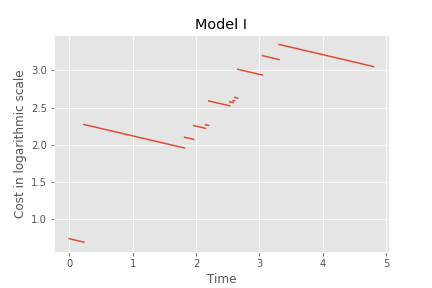
\includegraphics[scale=0.7]{img/model1.png}}
\caption{График U(t) для модели \rom{1}}
\end{figure}

Оптимальность данной стратегии исполнения, в частности, справедлива для бессрочного \textbf{колл-опциона} со \textbf{"страйком"} (ценой исполнения) $K$:

\begin{equation}\label{eq:payoff_function}
\Pi(s) = \max(s - K, 0) = (s - K)_+,
\end{equation}

Проблема состоит в том, чтобы сначала найти стоимость стратегии $T_L$. Будем рассчитывать её, как математическое ожидание приведённого к настоящему моменту платежа по опциону, то есть:

\begin{equation}\label{eq:strategy_cost}
V(s; L) = \expect*{e^{-rT_L} \Pi(S(T_L)) | S(0) = s}, s \le L,
\end{equation}

Здесь $T_L$ --- решающее правило предъявления опциона. С другой стороны, $T_L$ --- случайная величина, измеримая относительно $\sigma$ --- алгебры событий произошедших до момента $T_L$.

Затем определим оптимальное значение $\widetilde{L}$, которое максимизирует $V(s; L)$. Такое значение $\widetilde{L}$ --- оптимальная граница опциона. Итак, стоимость опциона равна:

\begin{equation}\label{eq:option_price}
    \begin{cases}
      V(s; \widetilde{L}), \text{ при } s \le \widetilde{L}\\
      \Pi(s), \text{ при } s > \widetilde{L}
    \end{cases}\,.
\end{equation}

\subsection{Свойства функции V(S)}

\begin{enumerate}
    \item Если $\Pi (s)$ не убывает, то и $V(s)$ не убывает. Например для функции платежа по колл-опциону:
    
    \begin{equation*}
        \Pi (s) = (s - K)_{+}
    \end{equation*}
    
    \item Если $\Pi (s)$ не возрастает, то и $V(s)$ не возрастает. Например для функции платежа по пут-опциону:
    
    \begin{equation*}
        \Pi (s) = (K - s)_{+}
    \end{equation*}
    
    \item Для всякого $s > 0$ следует, что $V(s) > \Pi (s)$.
    
    В самом деле, предъявляя опцион в момент $T_L = 0$, инвестор получает $\Pi (s)$
    
    \item Для колл- и пут- опционов $V(s) > 0$.
    
    Действительно, покажем это для пут-опциона с $\Pi (s) = (K - s)_{+}$. Для этого достаточно указать стратегию предъявления, при которой платёж положителен с положительной вероятностью.
    
    Для модели \eqref{eq:model1_definition} выберем $T$: $u - c T < ln K$.
    
    Будем предъявлять опцион в момент $T$ с вероятностью $e^{-\lambda T}$ на $[0, T]$ скачки $Z(t)$ не произойдут и $Z(T) = 0$. 
    
    Но при этом $S(T) = e^{u - c T} < e^{ln K} = K$ и $\Pi (S(T)) = K - S(T) > 0$.
    
    Аналогичный вывод можно сделать и для модели \eqref{eq:model2_definition}. Напомним, что $p(x)$, $x > 0$ --- плотность для случайной величины скачка $Y_i$. Для простоты доказательства предположим, что $p (x) > 0$ при $\forall x > 0$. Например, $p(x) = \beta e^{-\beta x}$ --- экспоненциальное распределение.
    
    Рассмотрим следующее решающее правило --- предъявлять опцион в момент скачка $T$, если $e^{U(T)} < K = e^{ln K}$. Но это событие произойдёт с положительной вероятностью уже при первом скачке, поскольку с положительной вероятностью этот скачок будет достаточно большим.
    
    \item Пусть $\Pi (S)$ не возрастает и $S_1 < S_2$. Если для функции платежа выполнено:

    \begin{equation*}
        \Pi (S_1) - \Pi (S_2) \le S_2 - S_1
    \end{equation*}
    
    то для стоимости опциона выполнено $V (S_1) - V (S_2) \le S_2 - S_1$.
    
    Примером подходящей функции будет $\Pi (S) = (K - S)^{+}$
    
    \item Пусть $\Pi (S)$ не убывает и $S_1 < S_2$. Если для функции платежа выполнено:

    \begin{equation*}
        \Pi (S_2) - \Pi (S_1) \le S_2 - S_1
    \end{equation*}
    
    то для стоимости опциона выполнено $V (S_2) - V (S_1) \le S_2 - S_1$.
    
    Примером подходящей функции будет $\Pi (S) = (S - K)^{+}$
\end{enumerate}

\section{Множество немедленного исполнения}\label{sec:immediate_execution}

Теперь мы можем вновь обратиться к обоснованию вида оптимальных пороговых правил. Определим множество немедленного исполнения:

\begin{equation*}
    \epsilon = \{S\textup{ | }V(S) = \Pi (S)\}
\end{equation*}

Оптимальное решающее правило:

\begin{equation*}
    \tau^{*} = \min\limits_{t} \{t\textup{ | }V(S(t)) = \Pi (S(t)) \}
\end{equation*}

Пусть $\Pi (S) = (K - S)^{+}$ --- пут-опцион. Тогда $\epsilon = (0, \tilde{L}]$, т.е. является полуинтервалом. В самом деле, если $S_2 \in \epsilon$ и $S_1 < S_2$, то и $S_1 \in \epsilon$. 

Действительно, имеем по свойству 5:

\begin{equation*}
    V (S_1) \le V(S_2) + S_2 - S_1 = K - S_2 + S_2 - S_1 = K - S_1 > 0
\end{equation*}

Но неравенство $V(S_1) \ge K - S_1$ следует из свойства 3. Значит:

\begin{equation*}
    V(S_1) = K - S_1,\ S_1 \in \epsilon
\end{equation*}

Поэтому $\tilde{L} = \max\limits_{S \in \epsilon} S$ и $\epsilon \in (0, \tilde{L}]$.

Пусть $\Pi (S) = (S - K)^{+}$, тогда $\epsilon = [\tilde{L}, +\infty)$. Доказательство данного факта аналогично. Значит, в рамках нашей задачи можем ограничиться пороговыми решающими правилами.

Для пут-опциона $T_L = \min\limits_{t}\{t\textup{ | }S(t) = L\}$. Среди них есть оптимальное правило $T_{\tilde{L}}$

%%%%%%%%%%%%%%%%%%%%%%%%%%%%%%%%%%%%
%%%%%% Решение для модели 1 %%%%%%%%
%%%%%%%%%%%%%%%%%%%%%%%%%%%%%%%%%%%%
\section{Решение для модели \rom{1}}

%%%%%%%%% Model II logarithmic track graph with cross with log(L)

\begin{figure}[htbp]
\label{fig:model1tracklcrosslog}
\centerline{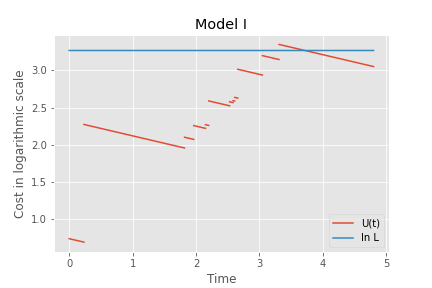
\includegraphics[scale=0.7]{img/model1_with_L_log.png}}
\caption{График пересечения U(t) и ln(L) для модели \rom{1}}
\end{figure}

%%%%%%%%% Model II track graph with cross with L

\begin{figure}[htbp]
\label{fig:model1tracklcross}
\centerline{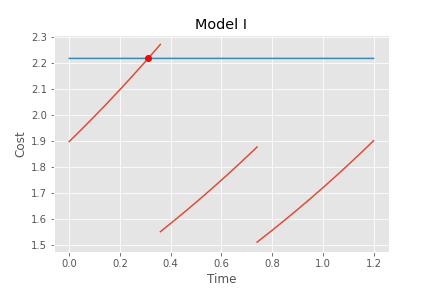
\includegraphics[scale=0.7]{img/model1_with_L.png}}
\caption{График пересечения S(t) и L для модели \rom{1}}
\end{figure}

Напомним, что модель \rom{1} определяется формулой \eqref{eq:model1_definition}:

\begin{equation*}
    U (t) = u + c t - Z(t)
\end{equation*}

Поскольку \hyperref[fig:model1tracklcross]{траектория} процесса $\{S(t)\}$ не имеет скачков вверх, точная нижняя грань \eqref{eq:optimal_excersize} достигается на непрерывном участке траектории. Это означает, что $S(T_L) = L$, и, следовательно, \eqref{eq:strategy_cost} получает вид:

\begin{equation}\label{eq:strategy_c1}
V(s; L) = \Pi(L) \expect*{e^{-rT_L} | S(0) = s}, s \le L,
\end{equation}

В \eqref{eq:strategy_c1} остается определить математическое ожидание. Для этого решим вспомогательную задачу --- найдём все такие $\xi$, при которых случайный процесс $\{e^{-rt}S(t)^{\xi}\}$ является мартингалом.

\begin{theorem}[Мартингальное условие для $\xi$]\label{thm:martingale_cond_for_xi}
Пусть для некоторого $\xi$, случайный процесс $\{e^{-rt}S(t)^{\xi}\}$ является мартингалом. Тогда мартингальное условие имеет вид:

\begin{equation}\label{eq:martingale_cond_for_xi_log}
\lambda \left[ \int_{0}^{+\infty} e^{\xi x} p(x) \,dx - 1  \right] - r - c \xi
 = 0
\end{equation}

\end{theorem}

\begin{proof}
Мартингальное условие для $\{e^{-rt} S(t)^{\xi}\}$:

\begin{equation*}
\expect*{e^{-rt} S(t)^{\xi}|S(0) = s} = s^{\xi}
\end{equation*}

Учитывая определение процесса $\{U(t)\}$:

\begin{equation*}
\expect*{e^{-rt + \xi U(t)}|U(0) = u} = e^{\xi u}
\end{equation*}

Так как $\{U(t), t \ge 0\}$ --- процесс с независимыми и стационарными приращениями, условие мартингальности для указанного процесса с произвольным $\xi$ при $t = 1$\footnote{выбор конкретного момента реализации процесса $t=1$ не сужает общности решаемой задачи} выглядит как:
\begin{equation*}\label{eq:thm2_eq1}
e^{-r}\expect*{e^{\xi U(1)}} = e^{\xi u}
\end{equation*}

Из формулировки первой модели \eqref{eq:model1_definition}, уравнение выше принимает вид:

\begin{equation*}
e^{-r}\expect*{e^{\xi(u + c - Z(1))}} = e^{\xi u}
\end{equation*}

Откуда можно вынести неслучайные составляющие:

\begin{equation*}
e^{-r + c \xi} \expect*{e^{-\xi Z(1)}} = 1
\end{equation*}

Заметим, что математическое ожидание в выражении выше представляет собой производящую функцию моментов обобщенного пуассоновского процесса\textsuperscript{{\ref{def:compound_poisson}}}:

\begin{equation*}
e^{-r + c \xi} M_{Z(1)}(-\xi) = 1
\end{equation*}

Теперь прологарифмируем обе части:

\begin{equation*}
\ln{M_{Z(1)}(- \xi)} - r + c\xi = 0
\end{equation*}

И применим результат леммы \ref{thm:thm2_moment_generating_function}:

\begin{equation*}
\ln{e^{\lambda (M_{Y_1}(- \xi) - 1)}} - r + c\xi = 0
\end{equation*}

Раскрыв логарифм, получим:

\begin{equation}\label{eq:thm2_eq2}
\lambda \left(M_{Y_1}(- \xi) - 1\right) - r + c\xi = 0
\end{equation}

Заметим, что $M_{Y_1}(-\xi)$, производящая функция моментов\textsuperscript{{\ref{def:moment_generating_function}}}, нам известна:

\begin{equation*}
M_{Y_1}(-\xi) = \expect{e^{-\xi Y_1}} = \int_{0}^{+\infty} e^{-\xi x} p(x) \,dx
\end{equation*}

Подставим производящую функцию моментов скачка в \eqref{eq:thm2_eq2} и получим требуемое:
\begin{equation*}
\lambda \left(\int_{0}^{+\infty} e^{-\xi x} p(x) \,dx - 1\right) - r + c\xi = 0
\end{equation*}
\end{proof}

Далее сформулируем утверждение о виде функции в левой части уравнения \eqref{eq:martingale_cond_for_xi_log}.

%%%%%%%%% Model I martingale condition

\begin{figure}[htbp]
\label{fig:model1martingalecond}
\centerline{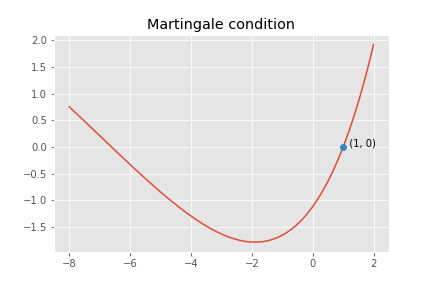
\includegraphics[scale=0.7]{img/model1_martingale_cond.png}}
\caption{Пример графика функции мартингального условия для модели \rom{1}}
\end{figure}

\begin{lemma}[Строгая выпуклость]\label{thm:strict_convexity_m1}
Выражение в левой части уравнения \eqref{eq:martingale_cond_for_xi_log} является строго выпуклой функцией по $\xi$.
\end{lemma}
\begin{proof}
Рассмотрим вторую производную данной функции:
\begin{equation*}
\begin{split}
     \pdv[2]{}{\xi} \left[\lambda \left(\int_{0}^{+\infty} e^{-\xi x} p(x) \,dx - 1\right) - r + c\xi \right] =\\
     = \pdv{}{\xi} \left[\lambda \left(\int_{0}^{+\infty} e^{-\xi x} p(x) x \,dx \right) + c \right] =\\
     = \lambda \left(\int_{0}^{+\infty} e^{-\xi x} p(x) x^{2} \,dx \right) &= \lambda \expect*{e^{-\xi x} x^2}
\end{split}
\end{equation*}

Так как $\lambda > 0$, $x^2 \ge 0$, $e^{-\xi x} > 0$, $p(x > 0) \neq 0$, выражение $\lambda \expect*{e^{-\xi x} x^2}$ строго положительно, как произведение положительной величины и математического ожидания ненулевой неотрицательной случайной величины. Итак, вторая производная исходной функции строго положительна.

\end{proof}

Учитывая положительность второй производной функции в уравнении \eqref{eq:martingale_cond_for_xi_log}, оно имеет не более двух решений. На самом деле, оно имеет ровно два решения.
\begin{lemma}[О числе решений уравнения \eqref{eq:martingale_cond_for_xi_log}]\label{thm:solution_for_mart_cond_m1}
Уравнение \eqref{eq:martingale_cond_for_xi_log} имеет ровно два решения. \\
Первое: $\xi_1 = 1$, \\
Второе: $\xi_2 = R > 0$, для некоторого $R$
\end{lemma}
\begin{proof}
Обозначим функцию в левой части уравнения \eqref{eq:martingale_cond_for_xi_log} через $f(\xi)$:
\begin{equation*}
f(\xi) = \lambda \left(\int_{0}^{+\infty} e^{-\xi x} p(x) \,dx - 1\right) - r + c\xi
\end{equation*}

Так как ${e^{-rt} S(T), t \ge 0}$ является мартингалом и в то же время является частным случаем процесса  $\{e^{-rt}S(t)^{\xi}\}$ при $\xi_1 = 1$, естественным образом получаем первое решение.

Существование второго решения следует из того, что:

\begin{equation*}
f(0) = \lambda \left(\int_{0}^{+\infty} e^{0} p(x) \,dx - 1\right) - r = \lambda (1 - 1) - r = -r
\end{equation*}

\begin{equation*}
\begin{split}
\lim_{\xi\to+\infty} f(\xi) &= \lim_{\xi\to+\infty} \left[ \lambda \left(\int_{0}^{+\infty} e^{- \xi x} p(x) \,dx - 1\right) - r + c\xi \right] =\\
= - \lambda - r + c \xi &= +\infty
\end{split}
\end{equation*}

А так как выражение в левой части --- непрерывная функция от $\xi$, она принимает все значения лежащие в $[min(f(\xi)), +\infty)$ на $\xi \in [0, +\infty)$ по теореме Больцано-Коши о промежуточном значении. Т.к. $min(f(\xi)) < 0$ (минимум достигается, причём не в $\xi = 1$, то есть $min(f(\xi)) < 0$), значит второе пересечение происходит в положительной полуоси: $\xi_2 = R > 0$, для некоторого $R$
\end{proof}

Отметим, что для положительного мартингала $\{e^{-rt} S(t)^{R}\}$ существует ограниченность сверху:

\begin{gather*}
    S(t) < L \\
    S(t)^{R} < L^R
\end{gather*}

Поэтому справедлива точная оценка по теореме о преобразовании свободного выбора:

\begin{equation*}
    \expect*{e^{-r T_L} S(T_L)^R | S(0) = s} = s^R
\end{equation*}

Учитывая $S(T_L) = L$:

\begin{equation*}
    \expect*{e^{-r T_L} S(T_L)^R | S(0) = s} = \expect*{e^{-r T_L} | S(0) = s} L^R
\end{equation*}

В результате имеем:

\begin{equation*}
    \expect*{e^{-r T_L} | S(0) = s} = \left(\frac{s}{L}\right)^{R}
\end{equation*}

Именно это математическое ожидание используется в формуле \eqref{eq:strategy_c1} для стоимости стратегии $T_L$, которую в данной статье мы обозначаем $V(s; L)$. В итоге получаем:

\begin{equation}\label{eq:strategy_c1_simplified}
V(s; L) = \left(\frac{s}{L}\right)^{R} \Pi(L), s \le L.
\end{equation}

Итак, нам удалось получить стоимость опциона. Максимизируем её для поиска оптимального порога. Вспомнив функцию $\Pi(S)$ по \eqref{eq:payoff_function}:

\begin{equation*}
\max\limits_{L} V(s; L) = \max\limits_{L} \left(\frac{s}{L}\right)^{R} (L - K), s \le L.
\end{equation*}

Осталось найти $\widetilde{L}$, то есть значение $L$, максимизирующее $V(s; L)$. Отметим, что $s^{R}$ есть некоторая константа, не зависящая от $L$. На деле нам нужно максимизировать $\frac{L - K}{L^R}$. Тогда условие первого порядка (теорема Ферма) имеет вид:

\begin{equation*}
    \pdv{}{L} \frac{L - K}{L^R} = \pdv{}{L} \frac{L^R - R L^R + R K L^{R-1}}{L^{2R}} = \pdv{}{L} \frac{(1 - R)L^R + R K L^{R-1}}{L^{2R}} = 0
\end{equation*}

После упрощения имеем:

\begin{equation*}
    (1 - R) L = - R K
\end{equation*}

Значит, формула для $\tilde{L}$:

\begin{equation}\label{eq:first_order_rule_m1}
    \tilde{L} = \frac{R}{1 - R} K
\end{equation}

А стоимость опциона из \eqref{eq:strategy_c1_simplified}:

\begin{equation*}
    \begin{cases}
       \left(\frac{s}{\widetilde{L}}\right)^{R} \Pi(\widetilde{L}), \text{ при } s \le \widetilde{L}\\
      \Pi(s), \text{ при } s > \widetilde{L}
    \end{cases}\,.
\end{equation*}

Или:

\begin{equation}\label{eq:option_price_m1}
    \begin{cases}
       \left(\frac{s}{\widetilde{L}}\right)^{R} (\widetilde{L} - K)_{+}, \text{ при } s \le \widetilde{L}\\
      s - K, \text{ при } s > \widetilde{L}
    \end{cases}\,.
\end{equation}

В следующем разделе представлен основной вклад этой статьи, оценивающий бессрочные опционы на активы, цены на которые могут перескакивать через оптимальную границу опциона-исполнения.

%%%%%%%%%%%%%%%%%%%%%%%%%%%%%%%%%%%%
%%%%%%% Решение для модели II %%%%%%
%%%%%%%%%%%%%%%%%%%%%%%%%%%%%%%%%%%%
\section{Решение для модели \rom{2}}

%%%%%%%%% Model II logarithmic track graph with cross with log(L)

\begin{figure}[htbp]
\label{fig:model2tracklcrosslog}
\centerline{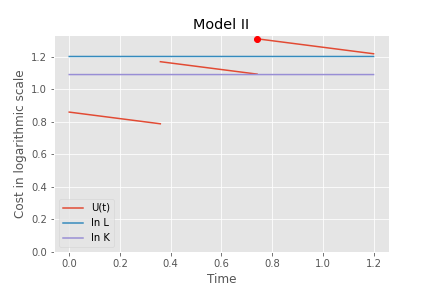
\includegraphics[scale=0.7]{img/model2_with_L_log.png}}
\caption{График пересечения U(t) и ln(L) для модели \rom{2}}
\end{figure}

%%%%%%%%% Model II track graph with cross with L

\begin{figure}[htbp]
\label{fig:model2tracklcross}
\centerline{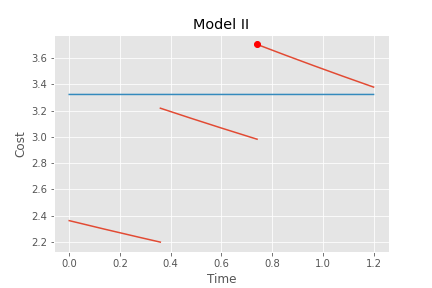
\includegraphics[scale=0.7]{img/model2_with_L.png}}
\caption{График пересечения S(t) и L для модели \rom{2}}
\end{figure}

\subsection{Мартингальный подход}

Как и прежде, мы ищем коэффициент $\xi$ такой, чтобы
процесс $\{e^{-rt + \xi U(t)}\}$ был мартингалом. В модели \rom{2} это приводит к условию:

\begin{equation}\label{eq:martingale_condition_for_mod2}
    \lambda \left[ \int_{0}^{+\infty} e^{\xi x} p(x) dx - 1 \right] - r + c \xi = 0
\end{equation}

Подобно \eqref{eq:martingale_cond_for_xi_log}, это уравнение имеет не более двух решений. Одно из них: $\xi_1 = 1$ (так как $\{e^{-rt} S(t)\}$ - мартингал).
При некоторых дополнительных условиях регулярности для плотности $p(x)$ уравнение имеет другое, положительное решение, $\xi_2 = R > 0$.

Вспомним, что в нашем случае моменты остановки ограничены:

\begin{equation*}
    T_L < \infty
\end{equation*}

Также отметим, что положительный мартингал $\{ e^{-r t} S(t)^R \}$ ограничен сверху при $t < T_L$:

\begin{equation*}
    e^{-r t} S(t)^R < S(t)^R < L^R
\end{equation*}

Тогда может быть применена теорема о преобразовании свободного выбора\textsuperscript{\ref{thm:OptSamplTheorem}}, которая дает:
\begin{equation}\label{eq:opt_sampl_applied_to_model2}
    \expect*{e^{-rT_L} S(T_L)^{R} | S(0) = s} = s^{R}
\end{equation}

Но теперь проблема в том, что $S(T_L) < L$ и что
распределение $S(T_L)$ вообще говоря неизвестно.

\subsection{Численный расчёт}

Определим численно для экспоненциального, гамма и логнормального уравнений решения уравнения \eqref{eq:martingale_condition_for_mod2}.

Рассмотрим подробнее интеграл в левой части этого уравнения:

\begin{equation*}
    \int_{0}^{+\infty} e^{\xi x} p(x) dx
\end{equation*}

Очевидно, что данный интеграл --- ни что иное, как производящая функция моментов $(\expect{e^{t X}})$. Для всех распределений сохраним постоянным математическое ожидание, обозначив его через $\mu$.

\subsubsection{Лог-нормальное распределение}

Для лог-нормального распределения данный интеграл расходится и нет возможности применить численный метод

\subsubsection{Гамма-распределение}

Для гамма-распределения, плотность распределения имеет вид:

\begin{equation}
    p(x) = \frac{1}{\Gamma(k) \theta^k} x^{k - 1} e^{-\frac{x}{\theta}},
\end{equation}

где $\Gamma (k) = (k - 1)!, \forall k \in \mathbb{N}$.

Производящая функция для гамма-распределения определена и имеет вид:

\begin{equation}
    MGF = \expect{e^{t x}} = (1 - \theta t)^{-k}, t < \frac{1}{\theta}
\end{equation}

Тогда наше уравнение \eqref{eq:martingale_condition_for_mod2} принимает вид:

\begin{equation*}
    \lambda \left[ (1 - \theta \xi)^{-k} - 1 \right] - r + c \xi = 0
\end{equation*}

С учётом фиксированного $\mu$ и формулы для математического ожидания гамма-распределения $\expect X = k \theta$:

\begin{equation*}
    \lambda \left[ \left(1 - \frac{\mu \xi}{k}\right)^{-k} - 1 \right] - r + c \xi = 0
\end{equation*}

\subsubsection{Экспоненциальное распределение}

Для экспоненциального распределения, плотность распределения имеет вид:

\begin{equation}
    p(x) = \frac{1}{\beta},
\end{equation}

Производящая функция для экспоненциального распределения определена и имеет вид:

\begin{equation}
    MGF = \expect{e^{t x}} = \frac{\beta}{\beta - t}, t < \beta
\end{equation}

Тогда наше уравнение \eqref{eq:martingale_condition_for_mod2} принимает вид:

\begin{equation*}
    \lambda \left[ \frac{\beta}{\beta - \xi} - 1 \right] - r + c \xi = 0
\end{equation*}

С учётом фиксированного $\mu$ и формулы для математического ожидания экспоненциального распределения $\expect X = \frac{1}{\lambda}$:

\begin{equation*}
    \lambda \left[ \frac{1}{1 - \xi \mu} - 1 \right] - r + c \xi = 0
\end{equation*}

\subsubsection{Результаты}

Сравним полученные результаты при запуске кода \ref{code:martingale_root} на разных значениях $\mu$. При этом $r = 10^{-2}$ и $c = 10^{-3}$ и поддерживались постоянными при всех опытах. 

\begin{table}[H]
\centering
\begin{tabular}{lll}
\rowcolor[rgb]{0.776,0.325,0.325} {\cellcolor[rgb]{0.875,0.624,0.624}}$\mu$ & $\xi_{gam}$                                    & $\xi_{exp}$                               \\
1000                                                                       & \textcolor[rgb]{0.129,0.129,0.129}{9.52e-05} & \textcolor[rgb]{0.129,0.129,0.129}{9.09e-05}  \\
500                                                                        & \textcolor[rgb]{0.129,0.129,0.129}{0.00019}  & \textcolor[rgb]{0.129,0.129,0.129}{0.00018}   \\
100                                                                        & \textcolor[rgb]{0.129,0.129,0.129}{0.00095}  & \textcolor[rgb]{0.129,0.129,0.129}{0.00091}   \\
50                                                                         & \textcolor[rgb]{0.129,0.129,0.129}{0.00189}  & \textcolor[rgb]{0.129,0.129,0.129}{0.00181}   \\
10                                                                         & \textcolor[rgb]{0.129,0.129,0.129}{0.00908}  & \textcolor[rgb]{0.129,0.129,0.129}{0.00908}   \\
5                                                                          & \textcolor[rgb]{0.129,0.129,0.129}{0.01732}  & \textcolor[rgb]{0.129,0.129,0.129}{0.01815}   \\
1                                                                          & \textcolor[rgb]{0.129,0.129,0.129}{0.06}     & \textcolor[rgb]{0.129,0.129,0.129}{0.09}      \\
0.5                                                                        & \textcolor[rgb]{0.129,0.129,0.129}{0.08}     & 0.18                                          \\
0.25                                                                       & \textcolor[rgb]{0.129,0.129,0.129}{0.09771}  & \textcolor[rgb]{0.129,0.129,0.129}{0.35196}   \\
0.125                                                                      & \textcolor[rgb]{0.129,0.129,0.129}{0.0999}   & \textcolor[rgb]{0.129,0.129,0.129}{0.6819}    \\
0.05                                                                       & \textcolor[rgb]{0.129,0.129,0.129}{1.5571}   & \textcolor[rgb]{0.129,0.129,0.129}{0.1}      
\end{tabular}
\end{table}

При этом стоит отметить, что при увеличении среднего значения, степень мартингала сходится к единому значению, отличаясь при $\mu = 1000$ лишь во 2 порядке точности. Это можно связать с тем, что при увеличении среднего значения вклад производящей функции моментов всё меньше, с другой стороны, и интересность решения численной задачи теряется.

\subsection{Экспоненциальный случай}

Примечательным исключением является случай, при котором величины скачка имеют экспоненциальное распределение, то есть $p(x) = \beta e^{-\beta x}$ для $x > 0$. Это распределение является распределением без памяти\textsuperscript{{\ref{def:memoryless_distr}}}, т.к. оно экспоненциальное.

\begin{theorem}\label{thm:jump_distribution_is_same}
Случайная величина $Y=U(T_L) - \ln L$ при условии $Y \ge 0$ и фиксированном $a = U(T_L^{-}) - \ln L < 0$ имеет то же экспоненциальное распределение, что и величина скачка $X_{T_L}=U(T_L) - U(T_L^{-})$. Здесь и далее $U(T_L^{-})$ --- момент непосредственно перед скачком.
\end{theorem}
\begin{proof}
Заметим, что:
\begin{equation*}
    Y = U(T_L) - \ln L = U(T_L) - U(T_L^{-}) + U(T_L^{-}) - \ln L = X(T_L) + a
\end{equation*}

Значит:
\begin{equation}\label{eq:y_distro_from_jump_proof}
    \mathbb{P}(Y > x \text{ | } S(T_L) > L) = \mathbb{P}(X(T_L) > x - a \text{ | } S(T_L) > L)
\end{equation}

Рассмотрим условие $S(T_L) > L$ подробнее:
\begin{gather*}
    S(T_L) > L \\
    U(T_L) > \ln L \\
    X(T_L) = U(T_L) - U(T_L^{-}) > \ln L - U(T_L^{-}) \\
    X(T_L) > \ln L - U(T_L^{-})
\end{gather*}

Воспользовавшись выражением для $a$:

\begin{equation*}
    X(T_L) > -a
\end{equation*}

Тогда наша условная вероятность в правой части \eqref{eq:y_distro_from_jump_proof} принимает вид:

\begin{equation*}
    \mathbb{P}(X(T_L) > x - a \text{ | } S(T_L) < L) = \mathbb{P}(X(T_L) > x - a \text{ | } X(T_L) > -a)
\end{equation*}

Используя свойство \textit{отсутствия памяти} у экспоненциального распределения (Подробнее: \ref{def:memoryless_distr}), получаем:

\begin{equation*}
    \mathbb{P}(X(T_L) > x - a \text{ | } X(T_L) > -a) = \mathbb{P}(X(T_L) > x)
\end{equation*}

Итак, совместив левый и правый элемент цепочки равенств, имеем искомое:
\begin{equation}\label{eq:y_distro_from_jump}
    \mathbb{P}(Y > x \text{ | } S(T_L) < L) = \mathbb{P}(X(T_L) > x)
\end{equation}

\end{proof}



Выразим теперь $S(T_L)$ через величину "перескока" через порог, обозначаемого через $Y$:

\begin{gather*}
    S(T_L) = e^{U(T_L)} \\
    S(T_L) = e^{(Y + \ln L)} \\
    S(T_L) = L e^Y
\end{gather*}

Подставим данное выражение для $S(T_L)$ в левую часть \eqref{eq:opt_sampl_applied_to_model2}:

\begin{equation*}
    \expect*{e^{-rT_L} (S(T_L))^{R} | S(0) = s} = \expect*{e^{-rT_L} (L e^Y)^{R} | S(0) = s}
\end{equation*}

Так как величина "перескока" и момент остановки $T_L$ независимы, можем записать 
\begin{equation*}
    \expect*{e^{-rT_L} (L e^Y)^{R} | S(0) = s} = \expect*{e^{-rT_L} | S(0) = s} \expect*{(L e^Y)^{R}}
\end{equation*}

Из этого и теоремы \ref{thm:jump_distribution_is_same} следует, что:

\begin{equation*}
\begin{split}
    s^{R} = \expect*{e^{-rT_L} | S(0) = s} \expect*{(L e^Y)^{R}} &= \\
    = \expect*{e^{-rT_L} | S(0) = s} \int_{0}^{+\infty} \beta (L e^{x})^{R} e^{-\beta x} dx &= \\
    = \expect*{e^{-rT_L} | S(0) = s} \beta \int_{0}^{+\infty} (L e^{x})^{R} e^{-\beta x} dx &= \\
    \expect*{e^{-rT_L} | S(0) = s} L^{R} \beta \int_{0}^{+\infty} e^{(R - \beta) x} dx
\end{split}
\end{equation*}

Заметим, что интеграл при $R - \beta \ge 0$ расходится, значит имеем в виду, что $R \ge \beta$:

\begin{equation}\label{eq:same_distr_conseq}
\begin{split}
    s^{R} = \expect*{e^{-rT_L} | S(0) = s} L^{R} \beta \int_{0}^{+\infty} e^{(R - \beta) x} dx &= \\
    = \expect*{e^{-rT_L} | S(0) = s} L^{R} \frac {\beta} {R - \beta}
\end{split}
\end{equation}

При этом из формулы \eqref{eq:strategy_cost} с учетом теоремы \ref{thm:jump_distribution_is_same} следует:

\begin{equation*}
    V(s; L) = \expect*{e^{-rT_L} \Pi(S(T_L)) | S(0) = s} = \expect*{e^{-rT_L} \Pi(L e^Y) | S(0) = s}
\end{equation*}

Так как момент остановки и величина перескока независимы:

\begin{equation*}
\begin{split}
    V(s; L) = \expect*{e^{-rT_L} \Pi(L e^Y) | S(0) = s} &= \\
    = \expect*{e^{-rT_L} | S(0) = s} \expect*{\Pi(L e^Y) | S(0) = s} &= \\
    = \expect*{e^{-rT_L} | S(0) = s} \beta \int_{0}^{+\infty} \Pi(L e^x) e^{-\beta x} dx
\end{split}
\end{equation*}

Учитывая \eqref{eq:same_distr_conseq} и факт выше в конечном итоге получаем, что:

\begin{equation}\label{eq:strategy_price_m2}
\begin{split}
    V(s; L) = \expect*{e^{-rT_L} | S(0) = s} \beta \int_{0}^{+\infty} \Pi(L e^x) e^{-\beta x} dx &= \\
    = \left( \frac{s}{L} \right)^R \frac{R - \beta}{\beta} \beta \int_{0}^{+\infty} \Pi(L e^x) e^{-\beta x} dx &= \\
    = \left( \frac{s}{L} \right)^R (R - \beta) \int_{0}^{+\infty} \Pi(L e^x) e^{-\beta x} dx &= \\
    = s^R (R - \beta) \cdot L^{-R} \int_{0}^{+\infty} \Pi(L e^x) e^{-\beta x} dx
\end{split}
\end{equation}

Чтобы определить оптимальную границу $\tilde{L}$ исполнения опциона, мы можем использовать два подхода. 

\textbf{Один} из них заключается в том, что $\tilde{L}$ должно максимизировать выражение:

\begin{equation*}
L^{-R} \int_{0}^{\infty} \Pi(L e^{x}) e^{-\beta x} dx
\end{equation*}

По принципу Ферма возьмём производную функции:

\begin{equation*}
\begin{split}
    \frac{\partial}{\partial L} \left[ L^{-R} \int_{0}^{\infty} \Pi(L e^{x}) e^{-\beta x} dx \right] &=\\
    = -R L^{-R-1}  \int_{0}^{\infty} \Pi(L e^{x}) e^{-\beta x} dx + L^{-R} \int_{0}^{\infty} \pdv{}{L} \Pi(L e^{x}) e^{x} e^{-\beta x} dx
\end{split}
\end{equation*}

Тогда условие стационарности в $\tilde{L}$ приводит к условию первого порядка:

\begin{equation}\label{eq:model2_first_idea_cond}
    \frac{-R}{\tilde{L}} \int_{0}^{\infty} \Pi(\tilde{L} e^{x}) e^{-\beta x} dx + \int_{0}^{\infty} \pdv{}{\tilde{L}} \Pi(\tilde{L} e^{x}) e^{(1 - \beta) x} dx = 0
\end{equation}

\textbf{Второй} заключается в том, что мы должны иметь:

\begin{equation}\label{eq:model2_second_idea_state}
    V(\tilde{L}; \tilde{L}) = \Pi(\tilde{L})
\end{equation}

Выполнение этого равенства означало бы, что функции $\Pi(s), s \le \tilde{L}$ и $V(s; \tilde{L}), s \ge \tilde{L}$ имеют непрерывное соединение в точке $s = \tilde{L}$. Уравнение \eqref{eq:model2_second_idea_state} при подстановке в \eqref{eq:strategy_price_m2} приводит к условию:

\begin{equation}\label{eq:model2_second_idea_cond}
\begin{split}
    V(\tilde{L}, \tilde{L}) = (\tilde{L})^R (R - \beta) (\tilde{L})^{-R} \int_{0}^{+\infty} \Pi((\tilde{L}) e^x) e^{-\beta x} dx &=\\
    = (R - \beta) \int_{0}^{+\infty} \Pi((\tilde{L}) e^x) e^{-\beta x} dx = \Pi(\tilde{L})
\end{split}
\end{equation}

Проведём \textbf{связь} между этими подходами. Интегрируя второй интеграл в \eqref{eq:model2_first_idea_cond} по частям, мы получим эквивалентность условий первого и второго подхода.

Условие непрерывного соединения может иметь следующее обоснование. Если $L$ --- таково, что $V(L; L) < P(L)$, мы делаем вывод, что $\tilde{L} > L$. Если, в обратном случае $L$ таково, что $V(L; L) > P(L)$, мы понимаем, что $\tilde{L} < L$. Таким образом мы мы показали, что $\tilde{L}$ должно удовлетворять \eqref{eq:model2_second_idea_state}. Также заметим, что это обоснование не учитывает ограничение на тот факт, что размер скачка имеет экспоненциальное распределение, а значит оно верно и в общем случае.

Таким образом, $\tilde{L}$ должно удовлетворять условию непрерывного соединения в общем случае. Для нашего же случая, когда $\Pi(S)$ --- известная функция, можно найти решение строго:

Из \eqref{eq:model2_first_idea_cond} и \eqref{eq:payoff_function}:

\begin{equation}\label{}
    - \frac{R}{\tilde{L}} \int_{0}^{\infty} \left((\tilde{L} e^{x} - K)_{+}\right) e^{-\beta x} dx + \int_{0}^{\infty} \pdv{(\tilde{L} e^{x} - K)_{+}}{\tilde{L}} e^{(1 - \beta) x} dx = 0
\end{equation}

Так как всюду, где $x < \ln K - \ln L$ платёжная функция равна $0$:

\begin{equation}
\begin{split}
    - \frac{R}{\tilde{L}} \int\limits_{\ln K - \ln L}^{\infty} \left((\tilde{L} e^{x} - K)\right) e^{-\beta x} dx + \int\limits_{\ln K - \ln L}^{\infty} \pdv{(\tilde{L} e^{x} - K)} {\tilde{L}} e^{(1 - \beta) x} dx &= \\
    = - \frac{R}{\tilde{L}} \int\limits_{\ln K - \ln L}^{\infty} \left((\tilde{L} e^{x} - K)\right) e^{-\beta x} dx + \int\limits_{\ln K - \ln L}^{\infty} e^{x} e^{(1 - \beta) x} dx &= \\
    = - \frac{R}{\tilde{L}} \int\limits_{\ln K - \ln L}^{\infty} \tilde{L} e^{(1 - \beta) x} dx - \frac{R K}{\tilde{L}} \int\limits_{\ln K - \ln L}^{\infty} e^{-\beta x} dx + \int\limits_{\ln K - \ln L}^{\infty} e^{(2 - \beta) x} dx &= \\
    = - \frac{R L e^{(1 - \beta) x}}{\tilde{L} (1 - \beta)}\bigg|_{\ln K - \ln L}^{\infty} + \frac{R K e^{-\beta x}}{\tilde{L} \beta}\bigg|_{\ln K - \ln L}^{\infty} - \frac{e^{(2 - \beta) x}}{2 - \beta}\bigg|_{\ln K - \ln L}^{\infty}
\end{split}
\end{equation}

Примем во внимание факт, что при $\beta < 2$ хотя бы один из интегралов расходится. При $\beta \ge 2$ несколько точек, а именно $\beta = 0$, $\beta = 1$, $\beta = 2$ не допускаются, т.к. дроби при них не определены

\subsubsection{Оптимальный порог при $\beta > 2$}

\begin{equation*}
\begin{split}
    - \frac{R L e^{(1 - \beta) x}}{\tilde{L} (1 - \beta)}\bigg|_{\ln K - \ln L}^{\infty} + \frac{R K e^{-\beta x}}{\tilde{L} \beta}\bigg|_{\ln K - \ln L}^{\infty} - \frac{e^{(2 - \beta) x}}{2 - \beta}\bigg|_{\ln K - \ln L}^{\infty} &= \\
    = \frac{R L e^{(1 - \beta) (\ln K - \ln L)}}{\tilde{L} (1 - \beta)} - \frac{R K e^{-\beta (\ln K - \ln L)}}{\tilde{L} \beta} + \frac{e^{(2 - \beta) (\ln K - \ln L)}}{2 - \beta} &= \\
    = \frac{R \left(\frac{K}{\tilde{L}}\right)^{(1 - \beta)}}{(1 - \beta)} - \frac{R K \left(\frac{K}{\tilde{L}}\right)^{-\beta}}{\tilde{L} \beta} + \frac{\left(\frac{K}{\tilde{L}}\right)^{(2 - \beta)}}{2 - \beta} = 0
\end{split}
\end{equation*}

Домножив обе части на $\left(\frac{K}{\tilde{L}}\right)^{\beta}$:

\begin{equation*}
    \frac{R \left(\frac{K}{\tilde{L}}\right)}{(1 - \beta)} - \frac{R K}{\tilde{L} \beta} + \frac{\left(\frac{K}{\tilde{L}}\right)^2}{2 - \beta} = 0
\end{equation*}

Обозначим за $x = \frac{K}{\tilde{L}}$:

\begin{equation*}
     \frac{x^2}{2 - \beta} + \frac{R x}{(1 - \beta)} - \frac{R x}{\beta} = 0
\end{equation*}

Так как $x \neq 0$:

\begin{equation*}
     x = (2 - \beta) \left(\frac{R}{\beta} - \frac{R}{(1 - \beta)}\right) = \frac{(1 - 2 \beta) (2 - \beta) R}{\beta (1 - \beta)}
\end{equation*}

В результате получаем оптимальный порог для экспоненциальной модели:

\begin{equation*}
    \tilde{L} = \frac{\beta (1 - \beta) K}{(1 - 2 \beta) (2 - \beta) R}
\end{equation*}

А стоимость опциона из \eqref{eq:strategy_price_m2}:

\begin{equation*}
\begin{cases}
    \left(\frac{s}{\widetilde{L}}\right)^R (R - \beta) \int_{0}^{+\infty} \Pi(L e^x) e^{-\beta x} dx, \text{ при } s \le \widetilde{L}\\
    \Pi(s), \text{ при } s > \widetilde{L}
\end{cases}\,.
\end{equation*}

Напомним, что опцион определён только для $\beta > 2$ и учтём формулу \eqref{eq:payoff_function}:

\begin{equation*}
\begin{cases}
    \left(\frac{s}{\widetilde{L}}\right)^R (R - \beta) \frac{K^{(1-\beta)}}{\beta (\beta - 1) L^{\beta}}, \text{ при } s \le \widetilde{L}\\
    s - K, \text{ при } s > \widetilde{L}
\end{cases}\,.
\end{equation*}

Упростив получим стоимость опциона для экспоненциально распределённых скачков вверх, то есть модели \rom{2}:

\begin{equation}\label{eq:option_price_m2_exp}
\begin{cases}
    \frac{s^R K^{1 - \beta} (R - \beta)}{L^{R + \beta} \beta (\beta - 1)}, \text{ при } s \le \widetilde{L}\\
    s - K, \text{ при } s > \widetilde{L}
\end{cases}\,.
\end{equation}

%%%%%%%%%%%%%%%%%%%%%%%%%%%%%%%%%%%%
%%%%%%%%%%%% Заключение %%%%%%%%%%%%
%%%%%%%%%%%%%%%%%%%%%%%%%%%%%%%%%%%%
\section{Заключение}

В этой статье рассматривается оценка бессрочных опционов, когда базовая акция следует смещенному сложному пуассоновскому процессу. В данной работе были рассмотрены две модели стоимости актива - со скачками вверх и со скачками вниз. В статье содержатся некоторые элегантные результаты.

В теории ценообразования опционов часто предполагается, что цена акции или фондового индекса следует геометрическому броуновскому движению. Оценка опциона, опирающегося на акцию или фондовый индекс, включает в себя анализ броуновского движения, который требует хорошего знания теории стохастических процессов и стохастического исчисления. С другой стороны, в актуарной науке долгое время применяли теорию распределения для моделирования страховых рисков и в результате распределения и преобразования широко используются и известны. Однако общая теория случайных процессов и стохастическое исчислением представляются более сложными. Мартингальный подход Гербера и Шиу позволяет нам решать некоторые проблемы ценообразования опционов, со сравнительно простым набором математических инструментов. Кроме того, это мощный инструмент для вычисления различных распределений времени столкновения с барьером геометрического броуновского движения. 

Как мы увидели, мартингальный подход обеспечивает простой аналитический метод без детального знания стохастического исчисления в отличие от классического метода.

Также были получены интересные и неожиданные результаты для экспоненциального распределения - вид функции стоимости опциона был разительно разным для двух моделей, что показало несимметричность модели со скачком вниз и модели со скачками вверх.

Исследование численных решений для гамма и экспоненциального распределений показали интересные разные степени для риск-нейтральных мартингалов, что результировало бы в ощутимо разные функции для стоимостей опционов.

Интересным продолжением данной работы могло бы стать исследование результатов для барьерных опционов с использованием данных моделей, а также гибридной модели, комбинирующей в себе и броуновское движение и модель со скачками, как модель \rom{1}* \cite{bib:GerberShiu}

%%%%%%%%%%%%%%%%%%%%%%%%%%%%%%%%%%%%
%%%%%%%%%%%% Литература %%%%%%%%%%%%
%%%%%%%%%%%%%%%%%%%%%%%%%%%%%%%%%%%%

\begin{thebibliography}{10}
\bibitem{bib:GerberShiu}
Gerber H.U., Shiu E.S.W. Pricing Perpetual Options for Jump Processes // North American Actuarial Journal --- 1998  v. 2, --- P. 108---109

\bibitem{bib:GARCH}
Bollerslev T. Generalized autoregressive conditional heteroskedasticity // Journal of Econometrics --- 1986  v. 31, --- P. 307---327

\bibitem{bib:Shiryaev}
Ширяев А.Н. О мартингальных методах в задачах о пересечении границ броуновским движением // Совр. пробл. матем. --- 2007 в. 8, --- с. 3–--78

\bibitem{bib:Shiryaev_Bulynski}
Булинский А.В,, Ширяев А.Н., "Теория случайных процессов // Физматлит --- 2006 в. 8, --- с. 3–--78

\bibitem{bib:Black_Scholes}
Black F., Scholes M. The Pricing of Options and Corporate Liabilities // The Journal of Political Economy --- 1973 v. 3, --- P. 637---654

\bibitem{bib:GerberShiu_Esscher}
Gerber H.U., Shiu E.S.W. Option pricing by Esscher transforms // Transactions of society of actuaries --- 1994 v. 46, --- P. 99---191

\bibitem{bib:GerberShiu_Actuarial_1}
Gerber H.U., Shiu E.S.W. An Actuarial Bridge
to Option Pricing // Securitization of Insurance Risk: The 1995 Bowles Symposium

\bibitem{bib:GerberShiu_Actuarial_2}
Gerber H.U., Shiu E.S.W. Actuarial Approach to Option Pricing // Proceedings AFIR --- 1995

\bibitem{bib:GerberShiu_Actuarial_3}
Gerber H.U., Shiu E.S.W. From Ruin Theory to Option Pricing // Actuarial Approach to financial risks --- 1998

\bibitem{bib:Perpetual_Mart1}
Gerber H.U., Shiu E .S. W. Martingale approach to pricing perpetual Аmеrican options on two stocks // Mathematical Finance --- 1996 v. 6, --- P. 303---322.
\bibitem{bib:Perpetual_Mart2}
Gerber H.U., Shiu E .S. W. Martingale approach to pricing perpetual Аmerican options // A STIN Bulletin. --- 1994. v. 24. --- P. 195---200.

\bibitem{bib:Musiela1997}
Musiela M., Rutkowski M. Modifications of the Black-Scholes Model // Springer Berlin Heidelberg. --- 1997 --- P. 135---158.

\bibitem{bib:BSModification}
Lin X., Wang M. A modification term for Black-Scholes model based on discrepancy calibrated with real market data // Data Science in Finance and Economics. --- 2021 --- P. 313---326.

\end{thebibliography}


%%%%%%%%%%%%%%%%%%%%%%%%%%%%%%%%%%%%
%%%%%%%%%%%% Приложение %%%%%%%%%%%%
%%%%%%%%%%%%%%%%%%%%%%%%%%%%%%%%%%%%
\appendix

\section{Код}

Задача поиска степени мартингала:\label{code:martingale_root}

\begin{lstlisting}
// solve.py

# Numeric solution to martingale condition

import math

import numpy as np
from matplotlib import pyplot as plt
from scipy.integrate import quad
from scipy.optimize import minimize

plt.rcParams["figure.figsize"] = [7.50, 3.50]
plt.rcParams["figure.autolayout"] = True

LAMBDA = 1e-1
R = 1e-2
C = 1e-3
MEAN = 0.9

# Generate equations for each distribution with relating parameters
def gen_gamma_eq(lmbd, r, c, theta, k):
    def gamma_eq(p):
        return lmbd * ((1 - theta * p) ** (-k) - 1) - r + c * p

    return gamma_eq


def gen_exp_eq(lmbd, r, c, beta):
    def exp_eq(p):
        return lmbd * ((beta) / (beta - p) - 1) - r + c * p

    return exp_eq


def solve_gamma(k=10):
    theta = MEAN / k
    eq = gen_gamma_eq(
        LAMBDA,
        R,
        C,
        k,
        theta,
    )
    t = minimize(
        lambda x: abs(eq(x)),
        -1,
        method="Nelder-Mead",
        constraints={"type": "ineq", "fun": lambda x: (1 - theta * x)},
        options={"xtol": 1e-10, "ftol": 1e-10, "maxiter": 1000},
    )

    assert t.x[0] < 1 / theta
    return t.x[0]


def plot_gamma(k=10):
    theta = MEAN / k
    eq = gen_gamma_eq(
        LAMBDA,
        R,
        C,
        k,
        theta,
    )

    x = np.linspace(-0.5, 0.5, 10000)
    plt.plot(x, eq(x), color="red")
    plt.show()


def solve_exp():
    beta = 1 / MEAN
    eq = gen_exp_eq(
        LAMBDA,
        R,
        C,
        beta,
    )
    t = minimize(
        lambda x: abs(eq(x)),
        -1,
        constraints={"type": "ineq", "fun": lambda x: beta - x},
        options={"xtol": 1e-10, "ftol": 1e-10, "maxiter": 1000},
    )
    assert t.x[0] < beta
    return t.x[0]


def plot_exp():
    beta = 1 / MEAN
    eq = gen_exp_eq(
        LAMBDA,
        R,
        C,
        beta,
    )
    x = np.linspace(-1, 1, 10000)
    new_eq = lambda x: np.nan if (abs(x - beta) < 1e-3) else eq(x)

    plt.plot(x, list(map(new_eq, x)), color="red")
    plt.show()


\end{lstlisting}

\end{document}
